%%%%%%%%%%%%%%%%%%%%%%%%%%%%%%%%%%%%%%%%%%%%%%%%%%%
%                                                 %
%                     SECTION                     %
%                                                 %
%%%%%%%%%%%%%%%%%%%%%%%%%%%%%%%%%%%%%%%%%%%%%%%%%%%

\section{Methodology}
\label{sec:sec004}

The hereby prototype used is the \hyperlink{https://github.com/mida-project/prototype-multi-modality-assistant/releases/tag/v1.0.1-alpha}{v1.0.1-alpha} version of our \hyperlink{https://github.com/mida-project/prototype-multi-modality-assistant/}{prototype-multi-modality-assistant}. The purpose of this prototype is to involve an \textit{AI-Assisted} tool (\textbf{Assistant}) for medical imaging at a breast screening diagnosis level. This \textbf{Assistant} was created with a front-end and bak-end architecture utilising common programming languages, libraries, frameworks and tools including \hyperlink{https://www.javascript.com/}{JavaScript (JS)}~\cite{flanagan2006javascript}, \hyperlink{https://nodejs.org/}{NodeJS}~\cite{wilson2018node}, \hyperlink{https://hammerjs.github.io/}{HammerJS}, \hyperlink{https://cornerstonejs.org/}{CornerstoneJS}~\cite{hostetter2018integration} and \hyperlink{https://www.orthanc-server.com/}{Orthanc}~\cite{Jodogne:ISBI2013}. For the Machine Learning (ML) and Deep Learning (DL)~\cite{ribeiro2017real, ribeiro2016real} component we will use several \hyperlink{https://www.mathworks.com/products/matlab.html}{MATLAB} technologies~\cite{vedaldi2015matconvnet}, promoting and feeding our Convolutional Neural Networks (CNN)~\cite{carneiro2015unregistered} and Deep Reenforcement Learning (DRL)~\cite{maicas2017deep} techniques. Other central component of this prototype is a web-based \hyperlink{https://www.sciencedirect.com/topics/medicine-and-dentistry/picture-archiving-and-communication-system}{PACS}~\cite{cooke2003picture} pairwise with ubicous web technologies and based on the \textbf{Open Source (OS)} \hyperlink{https://cornerstonejs.org/}{CornerstoneJS} library~\cite{feller2002understanding, hostetter2018integration}.

%%%%%%%%%%%%%%%%%%%%%%%%%%%%%%%%%%%%%%%%%%%%%%%%%%%
%                                                 %
%                     SECTION                     %
%                                                 %
%%%%%%%%%%%%%%%%%%%%%%%%%%%%%%%%%%%%%%%%%%%%%%%%%%%

\subsection{Environments}

This section describes the user environment over interaction, the so called \textbf{Radiology Room (RR)} (Figure \ref{fig:radioroom}). This guide is based on soft-copy diagnosis using computer workstations in their current reading room environment. It will be here where we take impressions regarding the efficacy of radiologists, and their recommendations based on their experience for improvements on the soft-copy reading environment. Several studies demonstrated~\cite{waite2017tired} that radiologist fatigue levels and performance are related to environmental factors such as number of false-negative and false-positives in addition to workstation enhancements. Supported by this guide, our research aims to conduct an investigation for the several environmental variables and improvements regarding the potentially enhancement that an \textit{AI-Assisted} diagnosis could take in the \textbf{RR}. We expect to analyse the needed information and best solution to improve the workstation results.

%%%%%%%%%%%%%%%%%%%%%%%%%%%%%%%%%%%%%%%%%%%%%%%%%%%

\hfill

\begin{figure}[h]
\centering
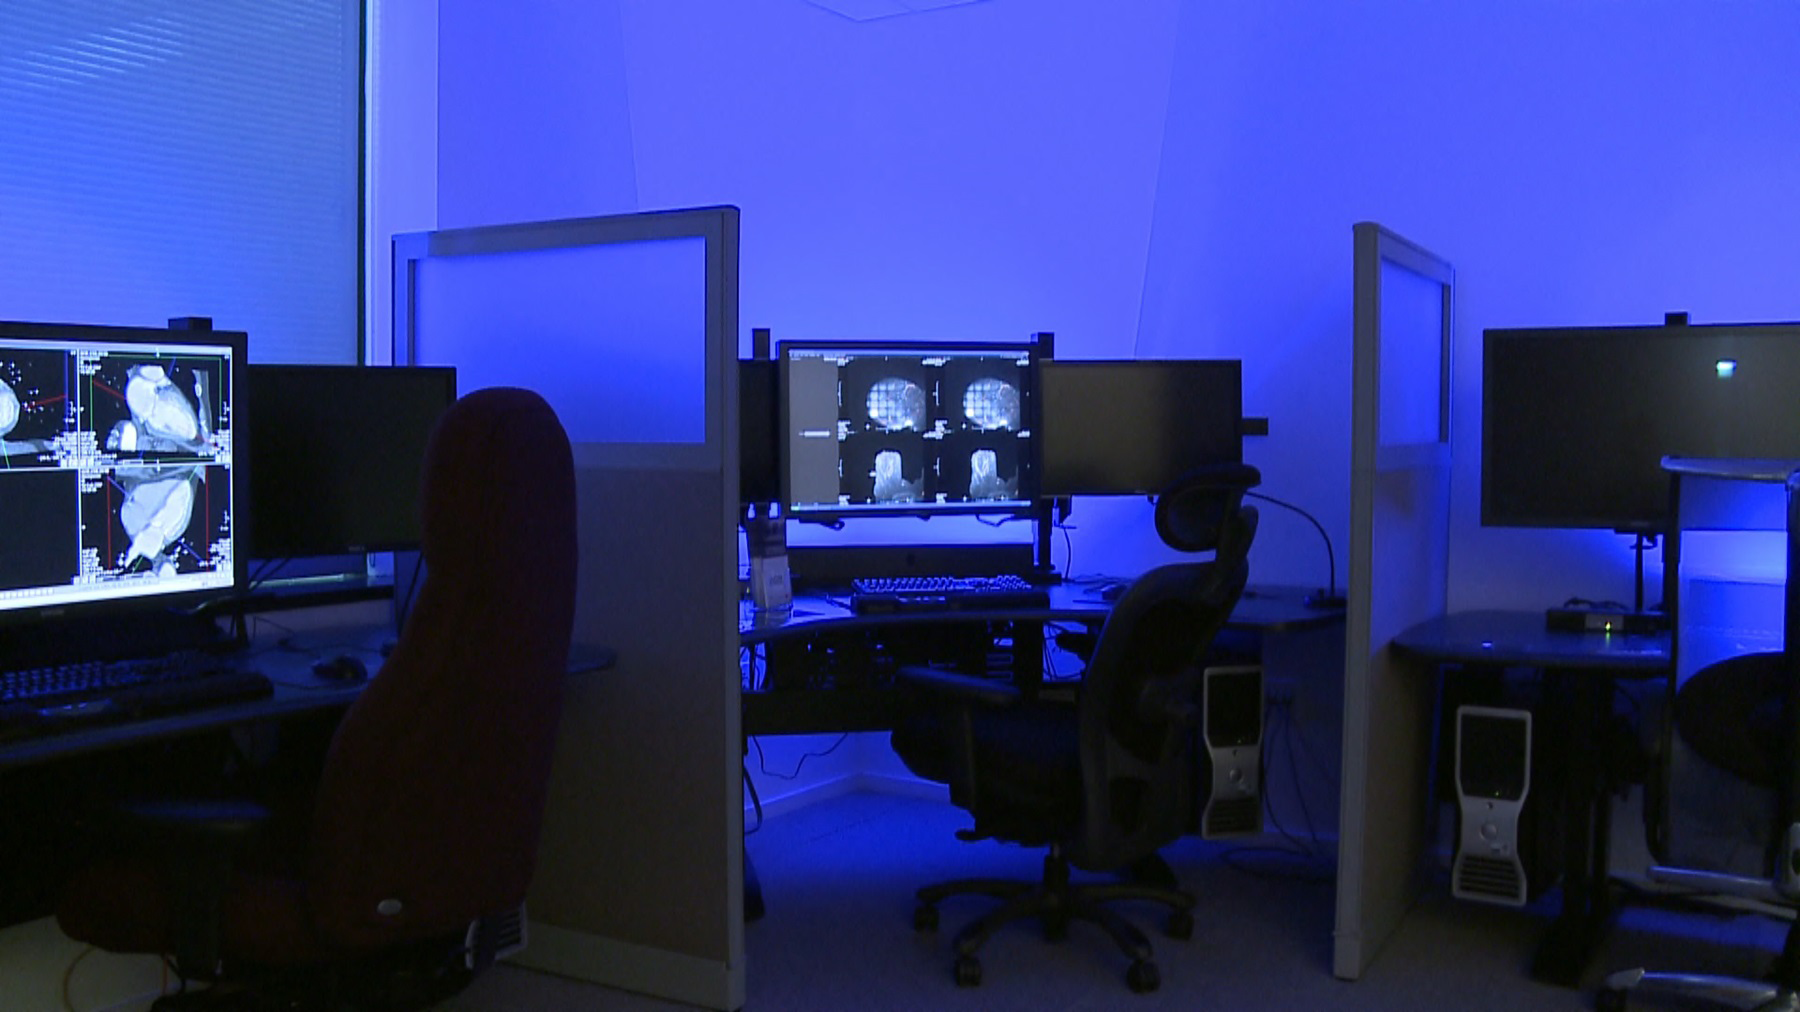
\includegraphics[width=\textwidth]{acr}
\caption{Radiology Room}
\label{fig:radioroom}
\end{figure}

\hfill

%%%%%%%%%%%%%%%%%%%%%%%%%%%%%%%%%%%%%%%%%%%%%%%%%%%

%%%%%%%%%%%%%%%%%%%%%%%%%%%%%%%%%%%%%%%%%%%%%%%%%%%
%                                                 %
%                     SECTION                     %
%                                                 %
%%%%%%%%%%%%%%%%%%%%%%%%%%%%%%%%%%%%%%%%%%%%%%%%%%%

\subsection{Case Studies}

The functionality of the prototype will be best demonstrated by a series of case studies. By describing the expected workflow and capabilities of the research study at the \textbf{RR} specific environment and changes of the workflow by using our system prototype. The study implies the evaluation of medical imaging \textit{AI-Assisted} features on several breast lesions. The primary goal of this case studies analysis is to generate a receiver operating characteristic to evaluate the performance and validation of our \textbf{Assistant}. Let us consider a list of hypothetical use cases for the research investigation that evaluates the interaction and usability performance of the \textbf{Assistant}. Therefore, the following list will show the preliminary case studies.

\hfill

List of case studies to analyse our solution prototype:

\hfill

\begin{itemize}
\item Multi-Modality \textit{AI-Assisted} of a Breast Cancer Diagnosis;
\item Priority \& Minimal Information Visualisation;
\item Performance \& Response Measurement Values Acquisition;
\item Radiologist Validation;
\end{itemize}

\hfill

%%%%%%%%%%%%%%%%%%%%%%%%%%%%%%%%%%%%%%%%%%%%%%%%%%%

We expect to demonstrate several uses through a series of case studies, including implementation of our research prototype using an \textit{AI-Assisted} technique and features for several view studies and other imaging research, as well as creation of a novel \textbf{Assistant} for the purpose. By creating a set of questions, we will try to achieve and feed this case studies. It is automatically associated with all cases. The radiologist may interact with our \textbf{Assistant} while manipulating the medical imaging and report to us difficulties and improvements. The number of questions is not restricted to the present document, since the interview will be open and suggestive~\cite{joyce2017healthcare}. There is no limit to the number of questions that can be asked per case but it should fit the amount of expected time per each.

The data will be collect from the study video and observations into a \hyperlink{https://docs.google.com/spreadsheets/d/1CoPLONnINdBWryGs7SBRuPZA-DnQ0t_yzx3u8ym0UoI/edit?usp=sharing}{spreadsheet} for further analysis. We will \hyperlink{https://github.com/mida-project/research-reports}{report} the results of this tests and conclusions. This guide and respective use cases will be iteratively improved.

\clearpage